\section{Analyse de l'additionneur}
Cette section présente une analyse théorique de la profondeur et du nombre de portes logiques dans les circuits additionneurs, construits à partir de cellules adders de 1 bit.

\subsection{1-bit Full Adder}
Une cellule d'additionneur complet de 1 bit prend trois entrées : $a_i$, $b_i$ (les bits à additionner) et $c_i$ (le carry-in). Elle produit deux sorties : $s_i$ (le bit de somme) et $c_{i+1}$ (le carry-out). Les expressions booléennes régissantes sont les suivantes :
\begin{align*}
    s_i &= (a_i \text{\textasciicircum} b_i) \text{\textasciicircum} c_i \\
    c_{i+1} &= (a_i \& b_i) | ((a_i \text{\textasciicircum} b_i) \& c_i)
\end{align*}
Ici, $\text{\textasciicircum}$ indique XOR, $\&$ indique AND, et $|$ indique OR.

\subsubsection{Profondeur logique (niveaux de porte)}
La profondeur logique est le nombre maximal de portes logiques connectées en série entre une entrée primaire (supposée au niveau 0) et une sortie.
\begin{itemize}
    \item \textbf{Sum $s_i$}:
    Le calcul implique deux opérations XOR séquentielles : $x_i = a_i \text{\textasciicircum} b_i$ (1er niveau de porte), suivi de $s_i = x_i \text{\textasciicircum} c_i$ (2ème niveau de porte). La profondeur logique de $s_i$ est de \textbf{2 niveaux de porte}.

    \item \textbf{Carry-out $c_{i+1}$} :
        Le chemin vers $c_{i+1}$ implique :
    \begin{enumerate}
        \item $p_i = a_i \& b_i$ (1er niveau de porte, AND).
        \item $x_i = a_i \text{\textasciicircum} b_i$ (1er niveau de porte, XOR, parallel a $p_i$).
        \item $q_i = x_i \& c_i$ (2ème niveau de la porte, AND, depend de $x_i$).
        \item $c_{i+1} = p_i | q_i$ (3ème niveau de la porte, OR, depend de $p_i$ et $q_i$).
    \end{enumerate}
     La profondeur logique de $c_{i+1}$ est de \textbf{3 niveaux de porte}.
\end{itemize}
La profondeur logique globale de la cellule de l'additionneur complet de 1 bit est déterminée par le chemin le plus long, qui va jusqu'à $c_{i+1}$, soit \textbf{3 niveaux de porte}.
\subsubsection{Nombre de portes logiques}
En supposant que les sous-expressions soient recalculées si elles sont utilisées dans des fonctions de sortie distinctes (par exemple, si les expressions de somme et de report sont analysées indépendamment, comme avec un utilitaire \texttt{parse\_parentheses}) :
\begin{itemize}
    \item For $s_i = (a_i \text{\textasciicircum} b_i) \text{\textasciicircum} c_i$: 2 XOR gates.
    \item For $c_{i+1} = (a_i \& b_i) | ((a_i \text{\textasciicircum} b_i) \& c_i)$: 1 XOR (pour $a_i \text{\textasciicircum} b_i$), 2 portes ET et 1 porte OU (4 portes au total pour la logique de report).
\end{itemize}
Le nombre total de portes logiques est de $2 + 4 = \textbf{6}$.

\subsection{Additionneur simple de $M$ bits}
Un additionneur simple de $M$ bits est formé par la mise en cascade de $M$ cellules de l'additionneur complet de 1 bit. La sortie $c_{i+1}$ de l'étage $i$ devient l'entrée de l'étage $i+1$. La retenue initiale, $c_0$, est généralement égale à  '0'.

\subsubsection{Profondeur logique (niveaux de porte)}
Le chemin critique qui détermine la profondeur est la propagation de la retenue du LSB(Least significant bit) au MSB(Most significant bit).
\begin{itemize}
    \item Stage 0 (LSB): Produces $c_1$ at a depth of 3 gate levels.
    \item Subsequent stages $i > 0$: The logic to produce $c_{i+1}$ from $c_i$ adds 2 gate levels to the path of $c_i$. Thus, $depth(c_{i+1}) = depth(c_i) + 2$.
    \item Tracing carry depths: $depth(c_1) = 3$; $depth(c_k) = 3 + (k-1) \times 2 = 2k + 1$.
    \item The final carry-out $c_M$ has $depth(c_M) = 2M + 1$.
    \item The MSB sum $s_{M-1}$ depends on $c_{M-1}$ (depth $2(M-1)+1$) and requires 2 more XOR levels, resulting in $depth(s_{M-1}) = (2(M-1)+1) + 2 = 2M+1$.
\end{itemize}
La profondeur logique d'un additionneur de $M$ bits est $\boldsymbol{D(M) = 2M + 1}$.\\
Par exemple :
\begin{enumerate}
    \item $M=1 \Rightarrow Profondeur=3$; 
    \item $M=2 \Rightarrow Profondeur=5$;
    \item $M=4 \Rightarrow Profondeur=9$.
\end{enumerate}


\subsubsection{Chemin le plus court (niveaux de porte)}
Le chemin logique le plus court est généralement celui de la somme LSB $s_0 = (a_0 \text{\textasciicircum} b_0) \text{\textasciicircum} c_0$. Cela implique \textbf{2 niveaux de porte} (deux XOR).

\subsection{Influence de la duplication des signaux sur la profondeur du graphe structurel}
Dans les représentations graphiques des circuits, les signaux (sorties de portes ou entrées primaires) servent souvent d'entrées à plusieurs portes ultérieures (split-out). Pour gérer cette situation, les structures des graphes comprennent des "nœuds de copie" (nœuds avec une étiquette vide \texttt{""}), qui dupliquent ou traversent les signaux.

L'introduction de ces nœuds de copie ajoute des couches structurelles au graphe. Alors que la profondeur logique ne prend en compte que la cascade de portes opérationnelles (AND, OR, XOR), la profondeur structurelle mesurée sur le graphe peut être plus importante. Chaque cas où un signal (par exemple, $a_i$, $b_i$, $c_i$) est acheminé vers plusieurs portes opérationnelles distinctes peut nécessiter une couche intermédiaire de nœuds de copie. Par conséquent, la profondeur structurelle globale du graphe, reflétant toutes ces couches opérationnelles et d'acheminement des signaux, peut dépasser la profondeur de la porte purement opérationnelle. Par exemple, pour un additionneur complet de 1 bit, la profondeur augmente de 2.

\begin{figure}[H]
    \centering
    \begin{minipage}{0.49\textwidth}
        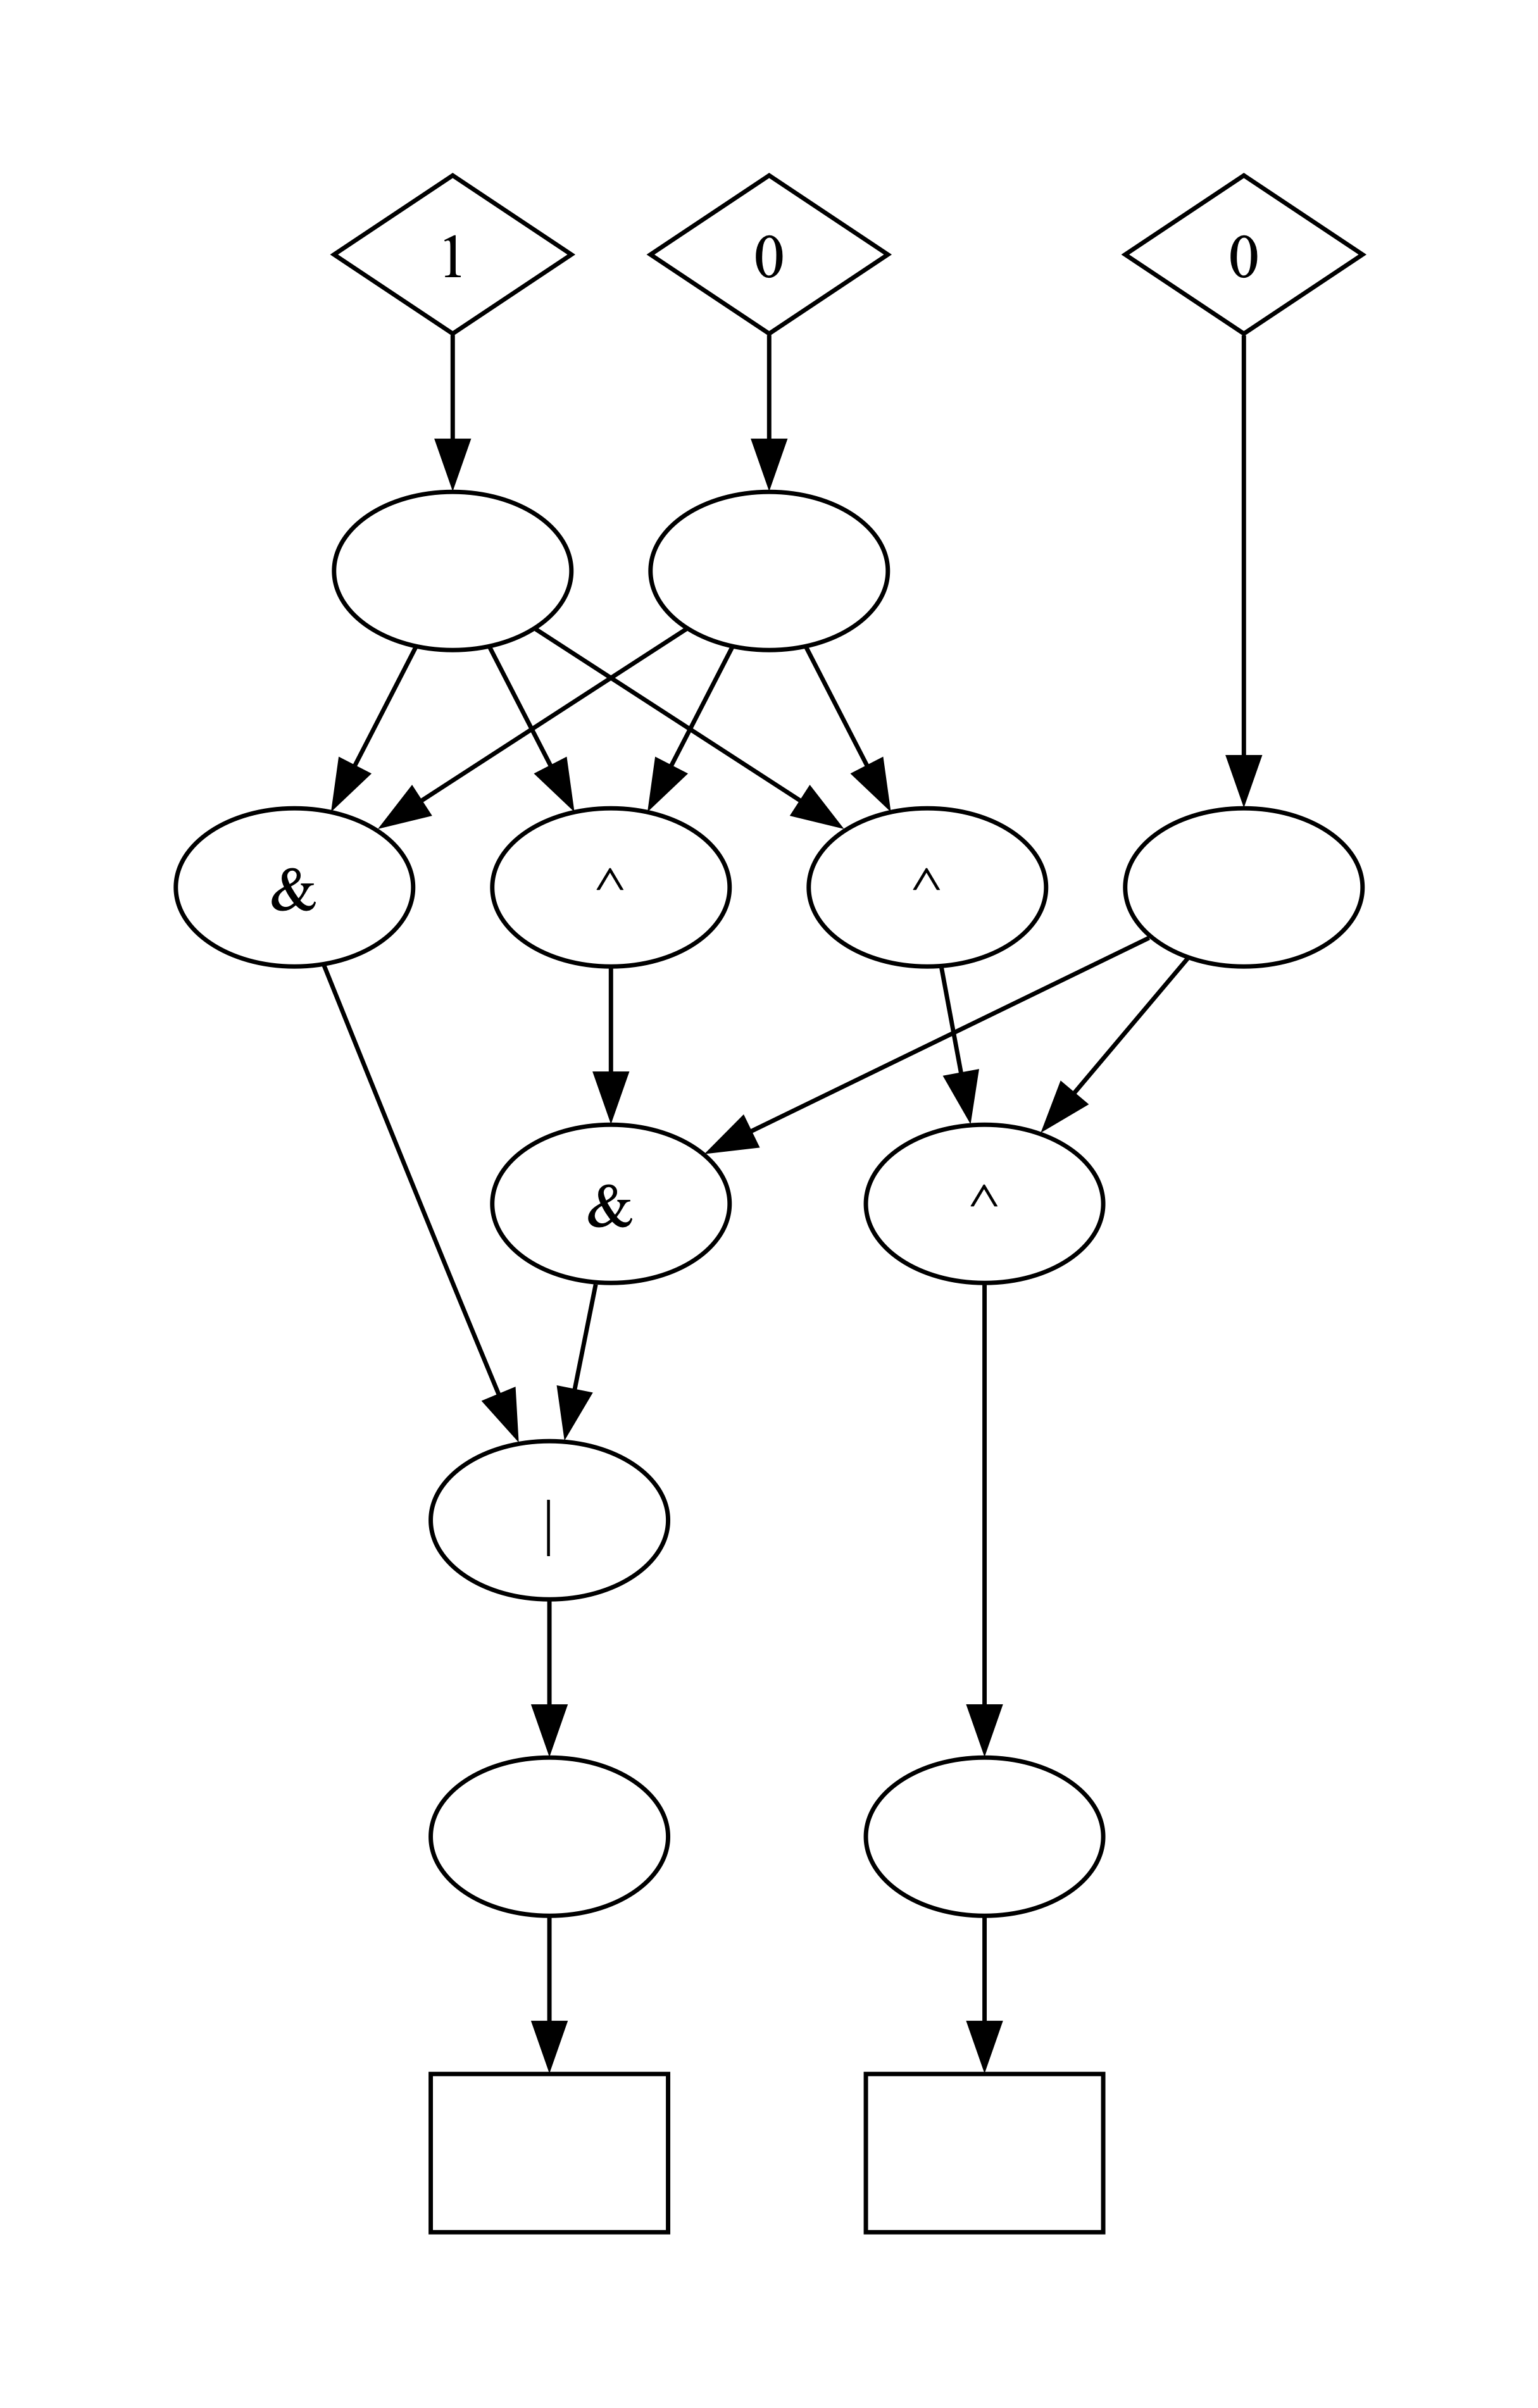
\includegraphics[width=0.8\textwidth]{figures/adder_1_bit.png}
    \end{minipage}
    \begin{minipage}{0.49\textwidth}
        \includegraphics[width=0.8\textwidth]{figures/adder_3_bit.png}
    \end{minipage}
    \caption{Exemples des adders des registres $2^0$ et  $2^1$ réspéctivement}
    \label{fig:}
\end{figure}

\section{Carry-Lookahead Adders}

L'additionneur de retenue (CLA) réduit la profondeur de calcul en pré-calculant les signaux de "propagation" ($P_i$) et de "génération" ($G_i$) pour chaque bit $i$ : $P_i = a_i \text{\textasciicircum} b_i$ et $G_i = a_i \& b_i$. Cela permet de déterminer les reports de manière plus directe. L'implémentation discutée utilise des blocs CLA de 4 bits, qui sont ensuite enchaînés pour des additionneurs plus grands de $4N$ bits.
\subsection{Analyse du bloc Carry-Lookahead 4 bits}
Un bloc de 4 bits traite les entrées $a_i, b_i$ (pour $i \in [0,3]$) et un \textit{carry-in} de bloc $C_{in_0}$, produisant les sommes $S_i$ et un \textit{carry-out} de bloc $C_{out_3}$ (également $C_4$).

\subsubsection{Génération des signaux P et G (bloc de 4 bits)}
\begin{itemize}
    \item \textbf{Nombre de portes :} 4 XORs (for $P_0..P_3$) + 4 ANDs (for $G_0..G_3$) = \textbf{8 portes}.
    \item \textbf{Profondeur logique :} Tous les $P_i, G_i$ sont calculés en parallèle : \textbf{1 niveau de porte}.
\end{itemize}

\subsubsection{Calcul de retenue (itératif dans un bloc de 4 bits)}
On utilise $C_{out,i} = G_i | (P_i \& C_{in,i})$, où $C_{in,i+1} = C_{out,i}$.
\begin{itemize}
    \item \textbf{Nombre de portes:} Pour 4 étapes ($C_{out,0}$ a $C_{out,3}$): $4 \times (1 \text{ AND} + 1 \text{ OR}) = \textbf{8 portes}$.
    \item \textbf{Profondeur logique :}
        
        $P_i, G_i$ sont à la profondeur 1. $C_{in,0}$ est à la profondeur 0.
        \begin{enumerate}
           
        \item $depth(C_{out,0})=3$ 
        \item $depth(C_{out,1})=5$
        \item $depth(C_{out,2})=7$
        \item $depth(C_{out,3})=9$.
        \end{enumerate}
        
   Le report de bloc $C_{out,3}$ est à \textbf{9 niveaux de porte}.
\end{itemize}

\subsubsection{Calcul de la somme (bloc de 4 bits))}
La somme des bits est calculée à l'aide de la formule $S_i = P_i \text{\textasciicircum} C_i$. La profondeur de chaque $S_i$ dépend des temps d'arrivée (profondeurs) de $P_i$ et $C_i$. Nous rappelons que tous les signaux $P_i$ sont disponibles à la profondeur 1, et que les porteuses $C_i$ (entrées de l'étage $i$) sont disponibles à des profondeurs variables : $C_0$ à la profondeur 0, $C_1$ à la profondeur 3, $C_2$ à la profondeur 5, et $C_3$ à la profondeur 7. La porte XOR pour $S_i$ ajoute un niveau à la profondeur maximale de ses entrées.

\begin{itemize}
    \item Pour $S_0 = P_0 \text{\textasciicircum} C_0$:
        $depth(S_0) = \max(depth(P_0), depth(C_0)) + 1 = \max(1, 0) + 1 = \textbf{2}$.
    \item Pour $S_1 = P_1 \text{\textasciicircum} C_1$:
        $depth(S_1) = \max(depth(P_1), depth(C_1)) + 1 = \max(1, 3) + 1 = \textbf{4}$.
    \item Pour $S_2 = P_2 \text{\textasciicircum} C_2$:
        $depth(S_2) = \max(depth(P_2), depth(C_2)) + 1 = \max(1, 5) + 1 = \textbf{6}$.
    \item Pour $S_3 = P_3 \text{\textasciicircum} C_3$:
        $depth(S_3) = \max(depth(P_3), depth(C_3)) + 1 = \max(1, 7) + 1 = \textbf{8}$.
\end{itemize}
La profondeur logique maximale parmi les sorties de la somme est pour $S_3$, qui est de \textbf{8 niveaux de porte}.

\subsubsection{Totaux pour un bloc CLA de 4 bits}
\begin{itemize}
    \item \textbf{Nombre total de portes logiques:} 8 (P/G) + 8 (Carry) + 4 (Sums) = \textbf{20 portes}.
    \item \textbf{Profondeur logique globale:} La profondeur déterminée est de \textbf{9 niveaux de porte} car pour la retenue, nous avons besoin de 9 niveaux de porte.
\end{itemize}


\subsubsection{Chemin le plus court (niveaux de porte)}
Il reste $S_0$ dans le premier bloc (LSB) : $\boldsymbol{2}$ niveaux de porte.

\subsection{Influence de la duplication des signaux sur la profondeur du graphe structurel (CLA)}
La construction directe de blocs CLA de 4 bits implique souvent des "nœuds de copie" comme dans l'additionneur simple. Ces nœuds non opérationnels augmentent la profondeur structurelle du graphe. Par exemple, un seul bloc CLA de 4 bits avec une profondeur logique de 9 peut présenter une profondeur structurelle de graphe plus élevée (15 lorsque l'on calcule la profondeur en utilisant le tri topologique du graphe).

\begin{figure}[H]
    \centering
    \includegraphics[width=0.8\textwidth]{figures/carry_lookahead_4.png}
    \caption{Exemple d'un carry look ahead}
    \label{fig:}
\end{figure}
